\documentclass[t,compress,xcolor=table]{beamer}
\mode<presentation>
\usetheme{Oxygen}
\setbeamertemplate{mini frames}[box] \usefonttheme[%
% % 	onlysmall, % headline, footline, and sidebars is changed
	onlylarge, % main title, frame titles, and section
]{structurebold}

\setbeamerfont*{frametitle}{size=\normalsize,series=\bfseries}

\hypersetup{pdfpagemode=FullScreen}

\usepackage[brazilian]{babel}
\usepackage{times}
\usepackage[T1]{fontenc}
\usepackage{hyperref}
\usefonttheme{serif}
\usepackage{fontspec}
\setsansfont{Bauhausb.ttf} 
\setmainfont{Verdana.ttf}
\usepackage{caption}
\usepackage{svg}
\usepackage{amsmath}
\usepackage{graphics}
\usepackage{graphicx}
\usepackage{pgf}			
\usepackage{multirow}	
\usepackage{tabularx}
\usepackage{wasysym}
\usepackage{lscape}
 \usepackage{booktabs}
\graphicspath{{./img/}}
\usepackage{graphicx}
\usepackage{bookmark}
% \usepackage[table,xcdraw]{xcolor}
%Comando de Subitem
\newcommand{\SubItem}[1]{
    {\setlength\itemindent{15pt} \item[-] #1}
}

% Setup TikZ
\usepackage{tikz}
\usetikzlibrary{arrows}
\tikzstyle{block}=[draw opacity=0.7,line width=1.4cm]

\newcommand{\plets}{$\textrm{PL}e\textrm{T}s$}

%\title[short title]{long title}
%\subtitle[short subtitle]{long subtitle}
%\author[short name]{long name}
%\date[short date]{long date}
%\institution[short name]{long name}

% Author, Title, etc.
\title[Extensionly]
{{\sffamily 
	Extensionly - Uma ferramenta de apoio à gestão de projetos e programas de extensão na universidade: Front end
}}

\author[Lucas Alexandre Fell]
{
	Lucas Alexandre Fell\inst{1} Maicon Bernardino\inst{1}
}

\date[Aug, 2022]{Alegrete, Brasil, 11/08/2022}

\institute[]
{
	\emph{lucasfell.aluno@unipampa.edu.br}\\
	\emph{bernardino@unipampa.edu.br}\\ 
	\vspace{7pt}
	\inst{1} Universidade Federal do Pampa (Unipampa)\\
	}

%\setbeamertemplate{footline}
%{
%	\leavevmode%
%	\hbox{%
%	
%	\begin{beamercolorbox}[wd=.25\paperwidth,ht=2.25ex,dp=1ex,center]{author in head/foot}%
%		%\usebeamerfont{author in head/foot}\insertshortauthor%~~(\insertshortinstitute)
%		\usebeamerfont{author in head/foot} iiWAS - 2013, Vienna, Austria
%		%Elder M. Rodrigues%~~(\insertshortinstitute)
%	\end{beamercolorbox}%
%	
%	\begin{beamercolorbox}[wd=.65\paperwidth,ht=2.25ex,dp=1ex,center]{title in head/foot}%
%		\usebeamerfont{title in head/foot}\inserttitle
%	\end{beamercolorbox}%
%	
%	\begin{beamercolorbox}[wd=.1\paperwidth,ht=2.25ex,dp=1ex,right]{date in head/foot}%
%		\usebeamerfont{date in head/foot} %\insertshortdate{}\hspace*{2em}
%		\insertframenumber{} / \inserttotalframenumber\hspace*{2ex}
%	\end{beamercolorbox}}%
%	
%	\vskip0pt%
%}

%####################################################################################

% The main document


\begin{document}

\begin{frame}[plain,t]
  \titlepage
\end{frame}

%######################################################################
\begin{frame}{{\sffamily Sumário}}

\begin{block}{}
	\begin{itemize}%[<+->]
	    \item Introdução
	        \SubItem{Motivação}
	        \SubItem{Questão de Pesquisa}
	        \SubItem{Objetivos} 
	        \SubItem{Contribuição} 
	    \item Metodologia
	        \SubItem{Metodologia de Pesquisa} % Adaptação
	        \SubItem{Desenho de Pesquisa} % BPMN
	\end{itemize}
\end{block}
\end{frame}
%######################################################################

%######################################################################
\begin{frame}{{\sffamily Sumário}}

\begin{block}{}
	\begin{itemize}%[<+->]
	    \item Contexto
	        \SubItem{Curricularização da extensão}
	        \SubItem{Programas e Projetos de extensão}
	       % \SubItem{Resoluções}
	        \SubItem{Unipampa Cidadã}
	    
	    \item Coleta de informações % Trabalhos Relacionados 
	        \SubItem{Busca na literatura cinza}
	        \SubItem{Levantamento (\textit{survey})}
	    
	\end{itemize}
\end{block}
\end{frame}

\begin{frame}{{\sffamily Sumário}}

\begin{block}{}
	\begin{itemize}%[<+->]
	    
	   \item Implementação
	        \SubItem{Perfis de Usuário}
	        \SubItem{Arquitetura}
	        \SubItem{Licença}
	        \SubItem{Estatísticas}
	    
	   \item Considerações Preliminares
	        \SubItem{Considerações Preliminares}
	        \SubItem{Lições Aprendidas} % e Relatos de Experiência
	        
	\end{itemize}
\end{block}
\end{frame}
% Introdução - descrever projeto em cooperação (front/back), extenso e feito em 2 mãos, estabelecer limites
% Motivação - SAP (unipampa), gestão da extensão, inexistência da gestão do projeto no sistema (emissão de certificados...) 
%=========================================
\chapter{Introduction}\label{introduction}
%=========================================

This work is part of a collaborative effort by two students from the Software Engineering course. Since the complexity and size of the problem were bigger than what the academy is used to seeing on \acp{TP}, the work was split among both authors. This decision was supported and previously agreed upon by their supervisor.

The effort was separated as follows: While this paper encompasses all of the front-end system requirements, such as analytics, multiple languages, component styling, design of the pages with the user interface and user experience, the counterpart focuses heavily on the back-end system requirements. Both projects are going to be separate implementations, will live in different version control repositories and both will have their own specific DevOps pipelines and deployments.

The \acl{UNIPAMPA} provides a number of options for students to engage in environments outside of the institution. An outreach activity can be defined as the following, in accordance with the 317th CONSUNI Resolution from April 29, 2021: An action that integrates the curriculum matrix and the organization of research, constituting an interdisciplinary, political, educational, cultural, scientific, and technological process \citeonline{res317}. Additionally, it fosters the development and use of knowledge in constant articulation with teaching and research, which transforms the interaction between \ac{UNIPAMPA} and society.

There are four (4) different modalities for outreach activities \citeonline{res317}:
\begin{inparaenum}[(i)]
  \item Program: a series of actions with a medium to long-term time frame that are focused on a single goal;
  \item Project: it is typically associated with a Program and has a clear goal and a set duration;
  \item Course: training activity, with short duration, and;
  \item Event: an action with an artistic, cultural and scientific character, with a well-defined duration.
\end{inparaenum}

As an illustration, consider the JEDI Program, which enlists the help of the local community (both academic and non-academic) as well as public or private businesses to address local issues and promote capacity building and IT training \cite{chamadaJedi}.

To register a new \ac{OA}, it is first necessary to identify whether it is a Specific or Linked \ac{OA} - whether it is linked to an Undergraduate Curriculum Component or not. The \ac{OA} insertion process is carried out at the \ac{PROEXT} of \ac{UNIPAMPA}. Once registered, the course committee will need to appoint one or more professors as outreach supervisors \cite{res317}.

The supervisor's duties also include creating and disseminating a biannual report detailing the outreach efforts conducted during the course, validating the use of Specific \acp{OA}, and evaluating the formative character of the action carried out by the student.

The student is responsible for requesting the use and validation of the hours spent in the activity with the Academic Secretary of the course after contacting the supervisor and expressing interest in an \ac{OA} \cite{res317}. Additionally, the professor is in charge of choosing and enrolling any student who expresses interest in the \ac{OA} program up until there are openings.

\section{Motivation}\label{sec:motivation}

It should come as no surprise that time is crucial in the academic setting. Because it is such a valuable resource, it needs to be handled with extreme caution. As there is currently no solution to handle all the requirements of generating and administering outreach programs in \ac{UNIPAMPA}, time is what propels this initiative forward.

The process of curricularization of the new \ac{OA} will be mandatedly implemented by \ac{HEI} in Brazil starting in 2023 as a result of Res. No317 \cite{res317}. However, the coordinator or other team members of the Outreach Programs and Projects would handle all management manually. In light of this, a number of problems with this manual method were found that might be easily resolved by adding a tool to assist the management process.

This implies that the professors and coordinators must personally complete everything, including constructing a project, submitting and getting it authorized, sending emails and making registration forms to open it for the students to join and eventually earn their participation certificate. Given the numerous emails the student receives from the institution each day, it is possible that one or more of the offers will go overlooked. The entire process is not optimized and requires a lot of time and work to complete.

Also due to the institutional program ``Unipampa Cidadã'' (Unipampa Citizen) - which aims to dedicate a portion of the hours currently invested in outreach activities in projects and areas of great social relevance - it is expected that the enrollment rate of new students in higher education will increase \cite{unipampacidada}, which consequently highlights even more the importance of automating manual processes at the university.

\section{Research Aims and Objectives}\label{sec:objectives}

According to what has been presented, this \ac{TP} has the research aim of developing the front-end part of a tool in which all the current management of \acp{OA} will be carefully observed and reproduced, in order to reduce the effort of the professors and supervisors with the manual steps of the process.

In order to achieve this, the following research objectives were defined:

\begin{itemize}
  \item Systematically review grey literature works and products in order to find similar solutions, collecting the first batch of requirements.
  \item Elaborate a survey, according to \citeonline{kasunic2005designing}, in order to discover new system requirements and in order to better understand the target users' needs.
  \item Analyze the results and refine the elicited requirements to create tangible tasks and an implementation roadmap.
  \item Study current market technologies, programming languages and frameworks to build a stack which delivers a great user experience and is creates a codebase that is easily maintained.
  \item Create a working \ac{MVP} of the system which implements at first the most critical collected and refined requirements for the system to become usable by early users to provide feedback for the product's further development \cite{becker_2020}.
\end{itemize}

\Cref{tbl:intro-objectives} also describes the research aim and questions.

\begin{table}[!htb]
  \centering
  \caption{Synthesis of the Research Aim and Research Objectives.}
  \label{tbl:intro-objectives}
  \footnotesize
  \begin{tabular}{l|p{11cm}}
    \bottomrule
    \rowcolor[rgb]{0.749,0.749,0.749} \multicolumn{1}{c|}{\textbf{Topic}}                  & \multicolumn{1}{c}{\textbf{Description}}                                                                                                                                                                                              \\
    \hline
    \rowcolor[rgb]{0.898,0.898,0.898} \textcolor[rgb]{0.145,0.145,0.145}{\textbf{Subject}} & Management of outreach programs and projects.                                                                                                                                                                                         \\
    \textbf{Study}                                                                         & Tool for Support in management of outreach programs and projects.                                                                                                                                                                     \\
    \rowcolor[rgb]{0.898,0.898,0.898} \textbf{Research Question}                           & How can a tool to support the management of outreach programs and projects of \acs{UNIPAMPA} optimize the management of proposition, registration, dissemination and accountability processes of outreach actions?                    \\
    \textcolor[rgb]{0.145,0.145,0.145}{\textbf{Research Hypothesis}}                       & With a tool to support the management of outreach programs and projects, it is possible to have a reduction on the effort needed to create an outreach activity and an increase in the engagement of volunteer outreach participants. \\
    \rowcolor[rgb]{0.898,0.898,0.898} \textbf{Research Aim}                                & Develop the front end of a tool to support the management of outreach programs and projects of \acs{UNIPAMPA}                                                                                                                         \\
    \textbf{Research Objectives}                                                           & Report results and execution methods of the following processes:
    \begin{inparaenum}[(i)]
      \item Research: Analyze similar tools, state the processes that will be made available by the tool, conduct surveys with the organizers and participants of \acp{OA}, understand the limitations of current processes.
      \item Planning: Elicitate functional and non functional requirements, identify stakeholders, define architecture and technologies.
      \item Development: Elaborate the features defined, build the entire front end.
      \item Deployment: Perform experiments with possible end users, collect feedback and implement appropriate improvements and corrections.
    \end{inparaenum}                                                                                                          \\
    \toprule
  \end{tabular}
  \fonte{Author.}
\end{table}

\section{Contribution}\label{sec:contribution}

The main contribution of this study will be the implementation of an \ac{MVP}, in the form of a web application, to support and automate the whole process of \acp{OA} in the university. It also aims to generate valuable artifacts about the state of outreach activities management tooling and support in Brazil, such as a grey literature review. A survey is also conducted, aiming to better understand the needs of outreach participants regarding this specific kind of tooling. Due to the complexity of this proposal, as previously mentioned, the effort was split amongst two \acp{TP}. This one focuses on the development of a web app, with all its related challenges, but it doesn't encompasses the back-end services in detail.

As for the artifacts generated to support the research, such as the grey literature systematic review and the survey, all of them were done in conjunction by both authors and are not related specifically to a single work. The other author is Igor Dalepiane da Costa.

\section{Organization}\label{sec:organization}

This document is organized according the following chapters:

\begin{itemize}
  \item \textbf{Chapter 2: Methodology}: Describes how the study was planned, the adopted methodology and the approaches used to conduct it.
  \item \textbf{Chapter 3: Background}: Important information and details of concepts related to the study, e.g. outreach activities in Brazil and in the \acl{UNIPAMPA}, federal laws and similar tools.
  \item \textbf{Chapter 4: Grey Literature}: How the protocol was structured, results, discovered tools, preliminary requirements.
  \item \textbf{Chapter 5: Survey}: How it was structured, results, validation of refined requirements with the target audience.
  \item \textbf{Chapter 6: Extensionly}: Revolves around implementation details, created artifacts, technologies used, the software engineering process, DevOps practices and the incorporation of analytics.
\end{itemize}

\section{Metodologia}
\subsection*{Metodologia}

\begin{frame}{{\sffamily Metodologia de Pesquisa}}
  \begin{block}{}
    Adaptação da classificação por Prodanov e Freitas:
    \begin{itemize}
      \item Abordagem qualitativa e quantitativa %
      \item Natureza aplicada: % Pesquisa aplicada, aplicar conhecimentos/resultados gerados em problemas específicos
            \SubItem{Geração de um produto}
      \item Quanto aos Objetivos: % Exploratória, utilizar os dois metodos para coletar informações para construir uma ferramenta melhor.
            \SubItem{Pesquisa exploratória}
      \item Quanto aos Procedimentos: %Documental literatura cinza, Estudo de caso coletar informações diretamente do usuário, Survey, teve teste piloto tbm.
            \SubItem{Documental - literatura cinza}
            \SubItem{Levantamento}
            \SubItem{Estudo de caso}

    \end{itemize}
  \end{block}
\end{frame}

\begin{frame}{{\sffamily Desenho de Pesquisa}}
  \begin{figure}
    \centering
    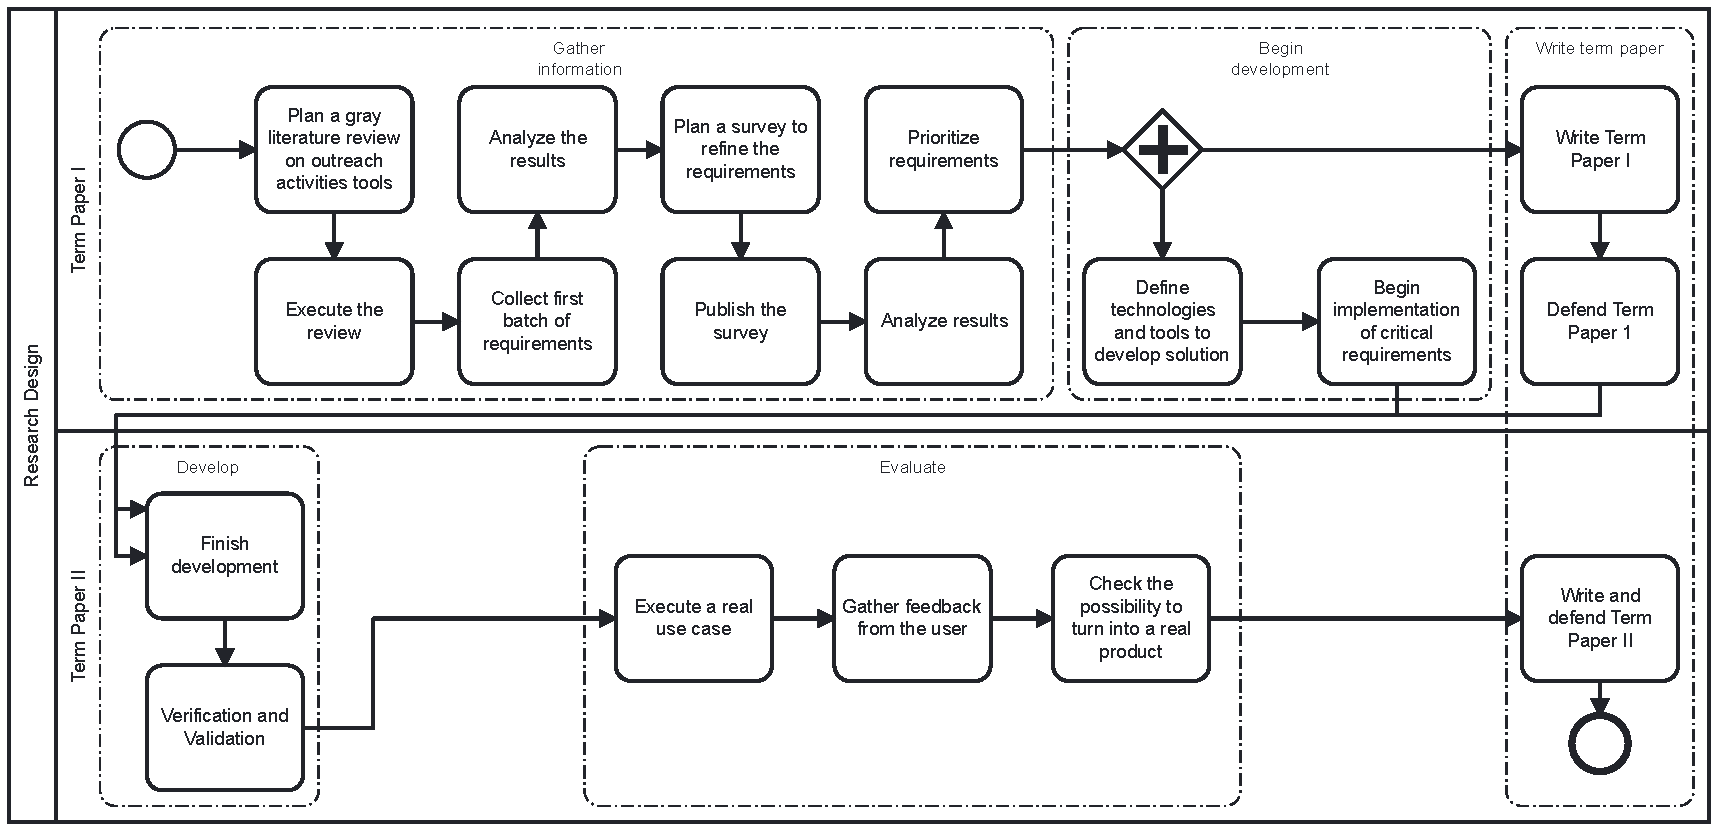
\includegraphics[width=11cm, ]{img/2-research design.pdf}
  \end{figure}
\end{frame}
% \item Contexto
% 	        \SubItem{Curricularização da extensão}
% 	        \SubItem{Resoluções}
% 	        \SubItem{Unipampa Cidadã}
%---------------------------------------------------------------------
\section{Contexto}
\subsection*{Contexto}
%---------------------------------------------------------------------

%######################################################################
\begin{frame}{{\sffamily Curricularização da Extensão}}
  \begin{block}{Legislação}
    \begin{itemize}
      \item Política Nacional de Extensão Universitária %Garantir q extensão pode resolver qualquer problema social, promover solidariedade tanto nacional como internacionalmente, reconhecer que extensão é uma peça essencial em universidades publicas;
            \SubItem{Extensão como solução para problemas sociais}
            \SubItem{Extensão como ferramenta essencial}
            \SubItem{Promover solidariedade e conscientização ambiental}
      \item Parte do curso como extensão (Res. 7 de 2018) %10% de horas, aumenta a procura e demanda
            \SubItem{10\% de horas do total}
            \SubItem{Adaptação em até 3 anos}
    \end{itemize}
  \end{block}
\end{frame}

\begin{frame}{{\sffamily Curricularização da Extensão na UNIPAMPA}}
  \begin{block}{Resoluções}
    \begin{itemize}
      \item Objetivos da extensão pela Res. 317 de 2021
            \SubItem{Desenvolver a educação crítica, cívica, interdisciplinar e responsável}
            \SubItem{Fortalecer o vínculo entre ensino, pesquisa e extensão}
      \item Formalização pela Res. 332 de 2021
            \SubItem{Órgãos gestores, participantes da extensão, tramitações}
      \item Cadeira de Resolução de Problemas
    \end{itemize}
  \end{block}
\end{frame}
%######################################################################

%######################################################################
\begin{frame}{{\sffamily Programas e projetos de extensão}}
  % Objetivo não é criar um laço de dependência entre comunidades, so para resolver um determinado problema e deixar que eles consigam andar com as proprias pernas depois, por isso a qualidade
  \begin{block}{O que são}
    Ações que envolvem ensino, pesquisa e a comunidade externa.
    \begin{itemize}
      \item Projetos possuem um objetivo específico e prazos determinados
      \item Um programa é um conjunto de projetos % Da pra falar das roles
    \end{itemize}
  \end{block}

  \begin{block}{Exemplos de programas}
    \begin{itemize}
      \item Programa C
      \item Programa JEDI
      \item Programa TRAMAS
    \end{itemize}
  \end{block}

\end{frame}

\begin{frame}{{\sffamily Unipampa Cidadã}}
  \begin{block}{}
    \begin{itemize}
      \item Extensão curricular
      \item Atividades solidárias % , 
            \SubItem{Campanha do agasalho, arrecadação de alimentos, suporte a asilos}
      \item Formação de egressos mais socialmente responsáveis % Egressos mais consientes com a responsabilidade social
      \item Oferecida por todos os cursos % 60 and a maximum of 120 hours
            \SubItem{Mínimo de 60 e máximo de 120 horas}
      \item Formulário de finalização da atividade.
    \end{itemize}
  \end{block}
\end{frame}
%######################################################################
\section{Revisão}
% Survey - lista preliminar da literatura -> validação com usuários reais, agregando novos requisitos
% protocolo, questionário, requisitos propostos, resultados, análise

%==============================================================================
\chapter{Survey}\label{survey}
%==============================================================================

\section{Survey protocol}\label{sec:sv-p}

\subsection{Pilot questionnaire}\label{sec:sv-p:pilot}

As \citeonline[p. 75]{kasunic2005designing} describes, a pilot test is a simulation of the real questionnaire carried out with a small number of members from the target audience. For this, the authors hand picked 7 (seven) people, out of which 4 (four) were students, 2 (two) were professors and 1 (one) was an \acl{TAE} (\ac{TAE}). The reason behind choosing this specific number of respondents is due to the following:
\begin{inparaenum}[(i)]
  \item All defined profiles for the respondents were chosen and
  \item the ratio of 4/2/1 is aligned with the expected numbers of submitted questionnaires per profile.
\end{inparaenum}

Unfortunately, the person chosen for the third profile, \ac{TAE}, wasn't able to answer. However, even though there are 3 (three) profiles, the questionnaire itself only has 2 (two) tracks of questions, one for students and the other for professors/\acp{TAE}. Because of that, the consequences of this happening weren't too impactful.

As for the pilot results, a lot of great feedback was received, along with some compliments on the organization of the questionnaire. There were issues with the person identification section, where the age was changed from a number to a range of numbers, such as between 21-29 years old.

\subsection{Distribute the Questionnaire}\label{sec:survey-distribute}

\section{Threats to validity}\label{sec:sv-validity}

% TAE didn't answer pilot test

\section{Results}\label{sec:sv-results}
\section{Implementação}

\section{Conclusão}

%######################################################################
% \begin{frame}{{\sffamily  Revisão Sistemática}}
%     \begin{figure}
%         \centering
%         \caption{Processo de Revisão Sistemática de Literatura (NAKAGAWA, E. et al.)} 
%         \includegraphics[width=0.68\textwidth]{Img/ProtocoloRS2.jpg}
%     \end{figure}
% \end{frame}
%######################################################################

% \begin{frame}{{\sffamily  Revisão Sistemática: Critérios de Inclusão}}
% \begin{block}{}
% 	\begin{itemize}%[<+->]
% 	        \item{CI1.O estudo deve citar uma ferramenta de teste de desempenho;}
% 	        \item{CI2.O estudo deve possuir avaliação empírica e expositiva sobre a ferramenta abordada;}
% 	        \item{CI3.Métricas e/ou padrões/normas de qualidade que apoiam a avaliação de uma ferramenta de teste de desempenho;}
% 	\end{itemize}
% \end{block}
% \end{frame}

% \begin{frame}{{\sffamily  Revisão Sistemática: Critérios de Exclusão}}
% \begin{block}{}
% 	\begin{itemize}%[<+->]
% 	        \item{CE1.Estudos duplicados;}
% 	        \item{CE2.O estudo não está escrito em inglês;}
% 	        \item{CE3.O estudo não fornece acesso completo ao seu conteúdo;}
% 	        \item{CE4.O estudo possui menos de 6 páginas, i.e., resumos expandidos;}
% 	\end{itemize}
% \end{block}
% \end{frame}

% \begin{frame}{{\sffamily  Revisão Sistemática: Goal Questions and Metrics}}
%     \begin{figure}
%         \centering
%         \includegraphics[width=0.95\textwidth]{Img/gqm.png}
%     \end{figure}
% \end{frame}

% \begin{frame}{{\sffamily  Revisão Sistemática: Questões de Pesquisa}}
% \begin{block}{}
% 	\begin{itemize}%[<+->]
% 	        \item{G1.Identificar quais são as ferramentas de teste de desempenho, e mapear suas funcionalidades.}
% 	        \SubItem{QP1.Quais são as ferramentas que apoiam o teste de desempenho?}
% 	        \SubItem{QP2.Quais as funcionalidades das ferramentas de teste de desempenho?}
% 	        \SubItem{QP3.Quais as abordagens de integração entre os artefatos de teste gerados nas ferra-mentas de teste de desempenho?}
% 	 \end{itemize}
% \end{block}
% \end{frame}

% \begin{frame}{{\sffamily  Revisão Sistemática: Questões de Pesquisa}}
% \begin{block}{}
% 	\begin{itemize}%[<+->]
% 	        \item{G2.Identificar abordagens, bibliotecas e ferramentas para visualização de dados,as quais possam ser utilizadas na análise de dados em relatórios de teste de desempenho.}
% 	        \SubItem{QP4.Quais as abordagens de apresentação dos resultados do teste de desempenho?}
% 	        \SubItem{QP5.Quais as abordagens de análise de resultados do teste de desempenho?}
% 	        \SubItem{QP6.Quais são as bibliotecas e ferramentas de visualização de dados a partir de uma entrada de dados?}
% 	 \end{itemize}
% \end{block}
% \end{frame}

% \begin{frame}{{\sffamily  Revisão Sistemática: Métricas}}
% \begin{block}{}
% 	\begin{itemize}%[<+->]
% 	        \item{M1.Nomes das ferramentas de teste de desempenho encontradas no estudo;}
% 	        \item{M2.Quais as funcionalidades das ferramentas;}
% 	        \item{M3.Abordagem de apresentação dos dados;}
% 	        \item{M4.Bibliotecas e ferramentas de visualização de dados.}
%     \end{itemize}
% \end{block}
% \end{frame}


% \begin{frame}{{\sffamily  Revisão Sistemática: String de Busca}}

% \begin{table}[!h]
% \centering
% \footnotesize
% \label{tab:DefinicaoSearch}
% \begin{tabular}{m{3cm}|m{6cm}}
% \bottomrule
% \rowcolor[HTML]{C0C0C0}
% \textbf{Termos} & \textbf{Sinônimos}
%  \\
% %\midrule 
% \rowcolor[HTML]{EFEFEF}
% \hline
% {\textbf{Performance Test}} & Load test, Stress test, Spike test, Workload test, Automation test 
%  \\
% %\midrule
% \hline
% \textbf{Tool} & Monitor, Generator, Plugin, Plug-in, Framework, Injector, Suite, Analyzer, Environment
% \\
% %\midrule
% \hline
% \toprule
% \end{tabular}
% \end{table}


% \begin{figure}[htb]
% \centering
% \fbox{\
% \normalsize
% \parbox{10cm}{
% \centering
% \scriptsize\texttt{
% (Performance test OR Load test OR Stress test OR Spike test OR Soak test OR Workload test OR Automation test) AND (Tool OR Monitor OR Generator OR Plugin OR Plug-in OR Framework OR Injector OR Suite OR Environment) AND (Software OR Application OR System)}}}
% \label{fig:StringBusca}
% \end{figure}

% \end{frame}

% \begin{frame}{{\sffamily  Revisão Sistemática: Estudos Primários}}
%     \begin{figure}[!h]
% 	\centering
% 	\caption{Estudos primários retornados nas bases de dados} 
% 		\includegraphics[width=.70\textwidth]{Img/ResultadosBases.JPG}
% 	\label{fig:ResusltadosBases}
% \end{figure}
%  \end{frame}

% % \begin{frame}{{\sffamily  Revisão Sistemática: Resultados dos Estudos Primários}}
% %     \begin{figure}
% %         \centering
% %         \includegraphics[width=0.99\textwidth]{Img/ResultadosBases.JPG}
% %         \end{figure}
% % \end{frame}

% \begin{frame}{{\sffamily  Revisão Sistemática: Processo de Seleção dos Estudos. }}
% \begin{figure}
%     \centering
%     \caption{Processo de Seleção dos Estudos.}
%     \includegraphics[width=0.70\textwidth]{Img/ciclos.PNG}
% \end{figure}
% \end{frame}

% % \begin{frame}{{\sffamily  Revisão Sistemática: Critérios de Qualidade}}
% % \begin{block}{}
% % 	\begin{itemize}%[<+->]
% %         \item{CQ1.Existem quaisquer declarações dos objetivos de pesquisa no estudo analisado?}
% %         \item{CQ2.O estudo apresenta características da ferramenta?}
% %         \item{CQ3.A proposta central do estudo está definida e é fortemente ligada às questões de pesquisa?}
% %         \item{CQ4.O estudo exibe as características e os recursos da análise dos resultados do teste de desempenho?}
% %         \item{CQ5.O estudo exibe detalhes de como é feita a integração dos artefatos gerados após o teste, para a análise dos resultados do teste de desempenho?}
% % 	\end{itemize}
% % \end{block}
% % \end{frame}

% \begin{frame}{{\sffamily  Revisão Sistemática: Avaliação de Qualidade}}
% \begin{figure}
%     \centering
%     \includegraphics[width=0.90\textwidth]{Img/qualidade.PNG}
% \end{figure}
% \end{frame}

% \begin{frame}{{\sffamily  Revisão Sistemática: Ferramentas Citadas nos Estudos}}
% \begin{figure}
%     \centering
%     \includegraphics[width=0.45\textwidth]{Img/ferramentas.PNG}
% \end{figure}
% \end{frame}

% \begin{frame}{{\sffamily  Revisão Sistemática: Funcionalidades das Ferramentas}}
% \begin{figure}
%     \centering
%     \includegraphics[width=0.52\textwidth]{Img/funcionalidades.PNG}
% \end{figure}
% \end{frame}

% \begin{frame}{{\sffamily  Revisão Sistemática: Formatos e Características do Relatório}}
% \begin{figure}
%     \centering
%     \includegraphics[width=0.35\textwidth]{Img/graficosferramentas.PNG}
% \end{figure}
% \end{frame}

% \begin{frame}{{\sffamily  Revisão Sistemática: Distribuição Geográfica dos Estudos}}
% \begin{figure}
%     \centering
%     \caption{Distribuição Geográfica dos Estudos} 
%     \includegraphics[width=0.95\textwidth]{Img/mapa.PNG}
% \end{figure}
% \end{frame}

% % \begin{frame}{{\sffamily  Revisão Sistemática: Anos de Publicação dos Estudos Selecionados.}}
% %     \begin{figure}
% %         \centering
% %         \includegraphics[width=0.70\textwidth]{Img/anosdepublicacao.PNG}
% %         \end{figure}
% % \end{frame}

% \begin{frame}{{\sffamily  Busca na Literatura Cinza: Motivação}}
%         \begin{block}{}
% 	\begin{itemize}%[<+->]
% 	    \item  Necessidade de encontrar ferramentas e bibliotecas de visualização de dados.
% 	    \item  \textit{Guidelines for including \textbf{Grey Literature} and conducting multivocal literature reviews in software engineering}. GAROUSI, V.
% 	    \end{itemize}
% \end{block}
% \end{frame}

% \begin{frame}{{\sffamily  Busca na Literatura Cinza: Ferramentas e Bibliotecas de Visualização de Dados}}
%     \begin{figure}
%         \centering
%         \includegraphics[width=0.33\textwidth]{Img/bibliotecas.png}
%         \end{figure}
% \end{frame}

% %######################################################################
% \section{Proposta}
% \subsection*{Proposta}
% %######################################################################


% \begin{frame}{{\sffamily  Requisitos}}
%     \begin{block}{}
% 	\begin{itemize}%[<+->]
% 	    \item  RQ1.A ferramenta precisa estar disponível sob licença open source.
% 	    \item  RQ2.A ferramenta tem de ser capaz de receber uma entrada de dados como parâmetro.
% 	    \item  RQ3.A ferramenta deve ser capaz de gerar gráficos a partir da entrada de dados.
% 	    \item  RQ4.A ferramenta deve ser capaz de apresentar dados de forma interativa.
% 	    \item  RQ5.A ferramenta deve automatizar a análise de resultados.
% 	\end{itemize}
% \end{block}
% \end{frame}

% \begin{frame}{{\sffamily Decisões de Projeto}}
%     \begin{block}{}
% 	\begin{itemize}%[<+->]
% 	    \item DP1. A ferramenta/biblioteca de visualização de dados deve ser \textit{open-source} (RQ1).
% 	    \item DP2. A ferramenta/biblioteca de visualização de dados deve ser capaz de receber uma entrada de dados (RQ2).
% 	    \item DP3. A ferramenta/biblioteca de visualização de dados tem de gerar gráficos a partir da entrada de dados (RQ3).
% 	\end{itemize}
% \end{block}
% \end{frame}

% \begin{frame}{{\sffamily Decisões de Projeto}}
%     \begin{block}{}
% 	\begin{itemize}%[<+->]
% 	    \item DP4. A ferramenta/biblioteca de visualização de dados deve possibilitar a apresentação de dados de forma interativa (RQ4).
% 	    \item DP5. A ferramenta deve fornecer alternativas para a análise de resultados automatizada (RQ5).
% 	\end{itemize}
% \end{block}
% \end{frame}

% \begin{frame}{{\sffamily  Arquitetura}}
%     \begin{figure}
%         \centering
%         \caption{Arquitetura da Proposta} 
%         \includegraphics[width=0.85\textwidth]{Img/arquiteturaearth.png}
%         \end{figure}
% \end{frame}

% \begin{frame}{{\sffamily  Diagrama de Caso de Uso}}
%     \begin{figure}
%         \centering
%         \includegraphics[width=0.75\textwidth]{Img/casodeuso.png}
%         \end{figure}
% \end{frame}

% \begin{frame}{{\sffamily  Caso de Uso 1. A ferramenta deve disponibilizar métricas \\para a análise dos resultados.}}
% \begin{figure}
%     \centering
%     \includegraphics[width=0.33\textwidth]{Img/earthresultados.PNG}
% \end{figure}
% \end{frame}

% \begin{frame}{{\sffamily  Caso de Uso 2. A ferramenta deve ser capaz de gerar \\gráficos a partir da entrada de dados}}
% \begin{figure}
%     \centering
%     \includegraphics[width=0.95\textwidth]{Img/earthnalysis.png}
% \end{figure}
% \end{frame}

% %######################################################################
% \section{Avaliação}
% \subsection*{Mapeamento das Necessidades}

% %######################################################################

% \begin{frame}{{\sffamily  Mapeamento das Necessidades}}
%     \begin{block}{}
% 	\begin{itemize}%[<+->]
% 	    \item  Planejamento;
% 	    \SubItem{Estrutura estabelecida}
% 	    \SubItem{Estratégia das questões}
% 	    \item  Objetivo;
% 	    \SubItem{Entendimento das necessidades da indústria}
% 	    \SubItem{Coletar informações de profissionais da área}
% 	    \item  Execução.
% 	    \SubItem{Distribuição do questionário}
% 	    \SubItem{52 participantes, 8 países*}
% 	\end{itemize}
% \end{block}
% \end{frame}
% %######################################################################

% %######################################################################

% \begin{frame}{{\sffamily  Mapeamento das Necessidades - Perfil dos Respondentes}}
% \begin{block}{}
% \begin{figure}
%     \centering
%     \includegraphics[width=0.25\textwidth]{Img/empresasmapeamento.png}
% \end{figure}
% \end{block}
% \end{frame}
% %######################################################################

% %######################################################################

% \begin{frame}{{\sffamily  Mapeamento das Necessidades - Nível Acadêmico}}
% \begin{block}{}
% \begin{figure}
%     \centering
%     \caption{Nível de formação acadêmica dos respondentes}
%     \includegraphics[width=0.85\textwidth]{Img/educacaomapeamento.png}
% \end{figure}
% \end{block}
% \end{frame}
% %######################################################################

% %######################################################################

% \begin{frame}{{\sffamily  Mapeamento das Necessidades - Nível de Experiência}}
% \begin{block}{}
%     \begin{figure}
%         \centering
%         \caption{Anos de Experiência na Indústria}
%         \includegraphics[width=0.85\textwidth]{Img/experienciamapeamento.png}
%     \end{figure}
%     \begin{figure}
%         \centering
%          \caption{Anos de Experiência como Engenheiro de Teste de Desempenho}
%         \includegraphics[width=0.85\textwidth]{Img/experienciatestermapeamento.png}
%     \end{figure}
% \end{block}
% \end{frame}
% %######################################################################

% %######################################################################

% \begin{frame}{{\sffamily  Mapeamento das Necessidades - Resultados}}
% \begin{block}{}
% 	\begin{itemize}%[<+->]
% 	    \item  Q1.\textit{How do you analyze the results of the performance test?} Do you use any tool? Which? (Como você analisa os resultados do teste de desempenho? Você usa alguma ferramenta? Qual?);
%             \SubItem{\textit{JMeter}, \textit{Dynatrace} e \textit{LoadRunner.}}
% 	    \item  Q2. \textit{What feature could help the process of analyzing the results?} (Que recurso poderia ajudar no processo de análise dos resultados?);
% 	        \SubItem{Gráficos, Comparação entre os testes executados, Customização, Visualização do tempo de resposta frente a outras métricas.}
% 	\end{itemize}
% \end{block}
% \end{frame}
% %######################################################################

% %######################################################################

% \begin{frame}{{\sffamily  Mapeamento das Necessidades - Questões Abertas}}
%     \begin{block}{}
% 	\begin{itemize}%[<+->]
% 	     \item  Q3. \textit{How do you rate the resources for analyzing results in performance testing tools?} (Como você classifica os recursos para análise de resultados em ferramentas de teste de desempenho?)
% 	     \item  Q4. \textit{How beneficial would be a solution that could be coupled with a performance test project, to have resources for the analysis of results?} (Quão benéfica seria uma solução que pudesse ser acoplada a um projeto de teste de desempenho, para ter recursos para a análise de resultados?)
% 	\end{itemize}
% \end{block}
% \end{frame}
% %######################################################################

% \begin{frame}{{\sffamily  Mapeamento das Necessidades - Questões Fechadas}}
% \begin{block}{}
% \begin{figure}
%     \centering
%     \caption{Classificação de 1 - 10 para pergunta \textbf{Q3.} e \textbf{Q4.}}
%     \includegraphics[width=0.95\textwidth]{Img/questoes.png}
% \end{figure}
% \end{block}
% \end{frame}
% %######################################################################

% \begin{frame}{{\sffamily  Mapeamento das Necessidades - Respostas}}
% \begin{block}{}
% 	\begin{itemize}%[<+->]
% 	    \item  Q5. \textit{Do you consider that generating graphs of the results is beneficial for the analysis of the results?} (Você considera que a geração de gráficos dos resultados é benéfica para a análise dos resultados?)
% 	\end{itemize}
% 	\begin{figure}
%         \centering
%         \includegraphics[width=0.95\textwidth]{Img/benefico.png}
%     \end{figure}
% \end{block}
% \end{frame}
% %######################################################################

% %######################################################################
% %\section{Avaliação}
% \subsection*{Avaliação Exploratória}

% %######################################################################

% \begin{frame}{{\sffamily Avaliação Exploratória}}
%     \begin{block}{}
% 	\begin{itemize}%[<+->]
% 	    \item  Planejamento;
% 	    \SubItem{Estrutura estabelecida}
% 	    \SubItem{Estratégia das questões}
% 	    \item  Objetivo;
% 	    \SubItem{Entendimento das necessidades da indústria}
% 	    \SubItem{Coletar informações de profissionais da área}
% 	    \item  Execução.
% 	    \SubItem{Distribuição do questionário}
% 	    \SubItem{15 participantes, 5 países*}
% 	\end{itemize}
% \end{block}
% \end{frame}
% %######################################################################

% %######################################################################

% \begin{frame}{{\sffamily Avaliação Exploratória - Perfil dos Respondentes}}
% \begin{block}{}
% \begin{figure}
%     \centering
%     \includegraphics[width=0.60\textwidth]{Img/empresasavaliacao.png}
% \end{figure}
% \end{block}
% \end{frame}
% %######################################################################

% \begin{frame}{{\sffamily  Avaliação Exploratória - Nível acadêmico}}
% \begin{block}{}
% \begin{figure}
%     \centering
%     \caption{Nível de formação acadêmica dos respondentes}
%     \includegraphics[width=0.85\textwidth]{Img/educacaoavaliacao.png}
% \end{figure}
% \end{block}
% \end{frame}
% %######################################################################

% \begin{frame}{{\sffamily  Avaliação Exploratória - Nível de Experiência}}
% \begin{block}{}
%     \begin{figure}
%         \centering
%         \caption{Anos de Experiência na Indústria}
%         \includegraphics[width=0.85\textwidth]{Img/experienciaavaliacao.png}
%     \end{figure}
%     \begin{figure}
%         \centering
%         \caption{Anos de Experiência como Engenheiro de Teste de Desempenho}
%         \includegraphics[width=0.85\textwidth]{Img/experienciatesteravaliacao.png}
%   \end{figure}
% \end{block}
% \end{frame}
% %######################################################################

% \begin{frame}{{\sffamily Avaliação Exploratória - Avaliação Técnica}}
%     \begin{block}{}
% 	\begin{itemize}%[<+->]
% 	    \item \textbf{QF1.} \textit{The tool help in analyzing performance test results.} (A ferramenta ajuda na análise dos resultados dos testes de desempenho.)
%         \item \textbf{QF2.} \textit{I would recommend this tool to a friend.} (Eu recomendaria esta ferramenta a um amigo.)
%         \item \textbf{QF3.} \textit{Using the tool can reduce the time spent analyzing the performance test results?} (O uso da ferramenta pode reduzir o tempo gasto analisando os resultados dos testes de desempenho?)
% 	\end{itemize}
% \end{block}
% \end{frame}
% %######################################################################

% \begin{frame}{{\sffamily Avaliação Exploratória - Avaliação Técnica}}
%     \begin{block}{}
% 	\begin{itemize}%[<+->]
%         \item \textbf{QF4.} \textit{Earthnalysis produce the expected graphs for the analysis of performance testing results.} (Earthnalysis produz os gráficos esperados para a análise dos resultados dos testes de desempenho.)
%         \item \textbf{QF5.} \textit{Using the tool can improve my performance when analyzing results of performance tests.} (O uso da ferramenta pode melhorar meu desempenho ao analisar resultados de testes de desempenho.)
%         \item \textbf{QF6.} \textit{The tool is fast in generating graphics and processing .CSV.} (A ferramenta é rápida na geração de gráficos e no processamento de .CSV.)
% 	\end{itemize}
% \end{block}
% \end{frame}
% %######################################################################

% \begin{frame}{{\sffamily  Avaliação Exploratória - Respostas}}
% \begin{block}{}
%     \begin{figure}
%         \centering
%         \caption{Respostas da Avaliação Técnica}
%         \includegraphics[width=0.85\textwidth]{Img/avaliacaotecnica.PNG}
%     \end{figure}
% \end{block}
% \end{frame}
% %######################################################################


% \begin{frame}{{\sffamily Avaliação Exploratória - Avaliação de Usabilidade}}
%     \begin{block}{}
% 	\begin{itemize}%[<+->]
%         \item \textbf{QU1.} \textit{Earthnalysis was easy to use.} (Earthnalysis foi fácil de usar.)
%         \item \textbf{QU2.} \textit{Earthnalysis is a good idea.} (Earthnalysis é uma boa ideia.)
%         \item \textbf{QU3.} \textit{I liked using Earthnalysis.} (Eu gostei de usar a Earthnalysis.)
%         \item \textbf{QU4.} \textit{Earthnalysis can facilitate the analysis of performance test results.} (Earthnalysis pode facilitar a análise dos resultados dos testes de desempenho.)
% 	\end{itemize}
% \end{block}
% \end{frame}
% %######################################################################

% \begin{frame}{{\sffamily  Avaliação Exploratória - Respostas}}
% \begin{block}{}
%     \begin{figure}
%         \centering
%         \caption{Respostas da Avaliação de Usabilidade}
%         \includegraphics[width=0.95\textwidth]{Img/avaliacaodeusabilidade.PNG}
%     \end{figure}
% \end{block}
% \end{frame}
% %######################################################################

% \begin{frame}{{\sffamily  valiação Exploratória - Questões Abertas}}
%     \begin{block}{}
% 	\begin{itemize}%[<+->]
% 	     \item \textbf{QA1.} \textit {What were the positive points in your experience with the tool?} (Quais foram os pontos positivos em sua experiência com a ferramenta?)
% 	        \SubItem{Facilidade de Uso, Intuitiva, Rápida geração de gráficos.}
% 	     \item \textbf{QA2.} \textit {What were the negative points in your experience with the tool?} (Quais foram os pontos negativos em sua experiência com a ferramenta?)
% 	        \SubItem{Interface muito simples, apenas um formato aceito como entrada de dados.}
% 	\end{itemize}
% \end{block}
% \end{frame}
% %######################################################################

% \begin{frame}{{\sffamily Avaliação Exploratória - Avaliação de Afeição}}
%     \begin{block}{}
% 	\begin{itemize}%[<+->]
% 	    \item \textit{Modelo do Circumplexo de Russell} 
%         \item \textbf{QR1.} \textit {Mood while performing the evaluation.} (Humor ao realizar a avaliação.)
%         \item \textbf{QR2.} \textit {Mood while using the tool.} (Humor ao usar a ferramenta.)
% 	\end{itemize}
% \end{block}
% \end{frame}
% %######################################################################

% %######################################################################

% \begin{frame}{{\sffamily  Avaliação Exploratória - Níveis de Afeição }}
% \begin{block}{}
%   \begin{figure}
%         \centering
%         \caption{Opções disponíveis para responder a QR1 e QR2.}
%         \includegraphics[width=0.99\textwidth]{Img/afeicao.PNG}
%     \end{figure}
% \end{block}
% \end{frame}
% %######################################################################

% %######################################################################

% \begin{frame}{{\sffamily  Avaliação Exploratória - Respostas}}
% \begin{block}{}
%   \begin{figure}
%         \centering
%         \caption{Humor enquanto executou a avaliação} 
%         \includegraphics[width=0.60\textwidth]{Img/russell.PNG}
%     \end{figure}
% \end{block}
% \end{frame}
% %######################################################################

% %######################################################################

% \begin{frame}{{\sffamily  Avaliação Exploratória - Respostas}}
% \begin{block}{}
% \begin{figure}
%     \centering
%     \caption{Humor enquanto utilizou a ferramenta} 
%     \includegraphics[width=0.55\textwidth]{Img/russell2.PNG}
% \end{figure}
% \end{block}
% \end{frame}
% %######################################################################

% \begin{frame}{{\sffamily Avaliação Exploratória - Ameaças à Validade do Estudo}}
%     \begin{block}{}
% 	\begin{itemize}%[<+->]
% 	    \item Validade do Constructo:
% 	        \SubItem{Criação de perguntas embasadas nos trabalhos relacionados.}
%         \item Validade Interna:
%             \SubItem{Estratégias para reduzir cansaço e desmotivação.}
%         \item Validade Externa:
%             \SubItem{Amostra representativa.}
%         \item Validade de Conclusão:
%             \SubItem{Estratégias para não ter um público enviesado.}
% 	\end{itemize}
% \end{block}
% \end{frame}
% %######################################################################


% %######################################################################
% \section{Considerações Finais}
% \subsection*{Considerações Finais}

% %######################################################################

% \begin{frame}{{\sffamily  Atividades Desenvolvidas}}
%     \begin{block}{}
% 	\begin{itemize}%[<+->]
% 	    \item  Levantamento do estado da arte;
% 	    \item  Elaboração da proposta;
% 	    \item  Desenvolvimento da ferramenta;
% 	    \item  Avaliação da ferramenta.
% 	\end{itemize}
% \end{block}
% \end{frame}

% %######################################################################

% \subsection*{Considerações Finais}

% %######################################################################

% \begin{frame}{{\sffamily  Lições Aprendidas e Relatos de Experiência}}
%     \begin{block}{}
% 	\begin{itemize}%[<+->]
% 	    \item Dificuldades encontradas;
% 	    \item Teste de desempenho na indústria;
% 	    \item Adesão na utilização da ferramenta desenvolvida.
% 	\end{itemize}
% \end{block}
% \end{frame}

% %######################################################################

% \begin{frame}{{\sffamily Earthnalysis - Uma Proposta de Visualização de Dados \\a partir de Relatórios de Teste de Desempenho}}
% \begin{block}{\begin{center}\huge{Perguntas?}\end{center}}
% 	\begin{center}
% 		\huge{}
% 	\end{center}
% \end{block}
% \begin{block}{Sobre:}
% 	\begin{itemize}%[<+->]
% 	    \item \href{http://lesse.com.br/}{{\color{blue}lesse.com.br}}
% 	    \item \href{http://novoportal.unipampa.edu.br/novoportal/}{{\color{blue}unipampa.edu.br}}
%     \end{itemize}
% \end{block}
% \end{frame}

% %######################################################################

\begin{frame}[plain,t]
  \titlepage
\end{frame}

\end{document}